% !TEX program = pdflatex
\documentclass[11pt]{article}
\setlength{\textwidth}{6.5in}
\setlength{\oddsidemargin}{0pt}
\setlength{\evensidemargin}{0pt}
\setlength{\textheight}{9in}
\setlength{\topmargin}{0pt}
\addtolength{\topmargin}{-\headheight}
\addtolength{\topmargin}{-\headsep}
\ifdefined\pdfpagewidth \pdfpagewidth=8.5in \pdfpageheight=11in \fi
\ifdefined\pagewidth \pagewidth=8.5in \pageheight=11in \fi
\usepackage{amsmath,amssymb}
\usepackage{array}
\usepackage{booktabs}
\usepackage[tableposition=top]{caption}
\usepackage{longtable}
\usepackage{enumitem}
\usepackage{tikz}
\usepackage{pgfplots}
\pgfplotsset{compat=1.18}
\emergencystretch=3em

% ---- notation ---------------------------------------------------------------
\newcommand{\um}{\,$\mu$m}
\newcommand{\kms}{km\,s$^{-1}$}
\newcommand{\flux}{erg\,cm$^{-2}$\,s$^{-1}$}
\newcommand{\mA}{m\AA}
\newcommand{\sci}[2]{#1\times10^{#2}}
\newcommand{\ion}[2]{#1\,\textsc{#2}}
\newcommand{\nuc}[2]{$^{#1}$#2}
\newcommand{\lxl}{$L_X/L_\mathrm{bol}$}

% ---- front matter -----------------------------------------------------------
\title{A Search for Ultraviolet Laser Lines\\ in Archival Spectra of Nearby Stars}
\author{Charles C. Norton}
\date{}

\begin{document}
\maketitle

\begin{abstract}
A laser aimed at Earth from another star adds an unresolved emission line to the
star's spectrum. We search the ultraviolet, where a diffraction-limited beam fills a
solid angle twenty times smaller than at visible wavelengths and cool stars are faint: $2356$ HST/STIS
echelle exposures of $530$ stars from StarCAT and $4312$ taken since, of $881$ stars,
$1138$ HST/COS far-ultraviolet spectra of $44$ stars within $10$\,pc, $851$ IUE
high-dispersion images of $58$ stars within $10$\,pc and $70$ FUSE observations of $42$
stars within $20$\,pc. A candidate is an
unresolved peak above the local upper envelope of the spectrum that recurs in a second
exposure, grating offset or detector channel and that fewer than two other stars show at
its rest or its observed wavelength, whether detected there or measured there directly.
No candidate remains. The features that persist in one star are narrow windows in the
line-blanketed spectrum of Arcturus at the wavelengths of its iron-group ions, emission
lines of the Mira R~Leo, the symbiotic EG~And and $\epsilon$~Eri,
lines of the crowded ultraviolet spectra of cool giants, T~Tauri stars, the Ap star
GY~And and the chromospheres of $\alpha$~Cen~A and B and Procyon, IUE features fixed to
one aperture's position on the camera, and IUE features
$440$\,\kms\ redward of the \ion{Si}{ii} $1808$ and $1817$\,\AA\ lines of the brightest
G and K dwarfs, which the STIS spectrum of $\alpha$~Cen~A excludes. Lines injected into
the archival spectra and recovered by the same detectors give the sensitivity. At the
stars within $10$\,pc the median limit for an isotropic source is $\sci{2.0}{17}$\,W
with COS and $\sci{1.0}{18}$\,W with the later STIS spectra, and a transmitter aimed at
Earth through a diffraction-limited $10$\,m aperture, whose beam at $1200$\,\AA\ is
$0.005$\,au wide at the nearest stars, would have been detected at $0.1$
to $7$\,W from $21$ of the $27$ stars within $5$\,pc, at $0.11$\,W from Lalande~21185
and $0.14$\,W from Barnard's star.
\end{abstract}

% =============================================================================
\section{Introduction}\label{sec:intro}
% =============================================================================

Schwartz and Townes proposed that a civilization could signal with optical masers,
whose light, confined to a narrow beam and a narrow band, would outshine its star at
that wavelength~\cite{SchwartzTownes1961}. A laser aimed at Earth from another star
would add an unresolved emission line to the star's spectrum, and spectroscopic searches
for such lines have examined optical spectra of nearby stars: $577$ FGKM stars with
Keck/HIRES at $4000$--$5000$\,\AA~\cite{ReinesMarcy2002}, $2796$ stars at
$3640$--$7890$\,\AA~\cite{TellisMarcy2015}, $5600$ FGKM stars with thresholds of
megawatts~\cite{TellisMarcy2017}, $1983$ spectra of $388$ stars from the Automated
Planet Finder~\cite{Zuckerman2023}, and $2821$ stars in archival HARPS
spectra~\cite{FieldsGoodman2025}.

The ultraviolet favours such a transmitter in two ways. A diffraction-limited beam from
an aperture $D$ fills a solid angle of about $(\lambda/D)^2$, so at $1200$\,\AA\ an
aperture puts its power into a solid angle twenty times smaller than at $5500$\,\AA;
from $10$\,m the beam is $0.005$\,au wide at $2$\,pc and $0.025$\,au at $10$\,pc, far
narrower than the Earth's orbit, so the transmitter must be aimed at the Earth itself,
at its position when the light arrives, and not at the Sun. And
the photospheres of K and M dwarfs, the commonest nearby stars, emit almost no
far-ultraviolet continuum, so a line of given power stands out against far less light.
The cost is that the atmosphere absorbs the ultraviolet, so only a receiver in space sees
the signal, and that the interstellar medium absorbs the Lyman series and the resonance
lines of abundant ions. Within $10$ to $20$\,pc the hydrogen column is of order
$10^{18}$\,cm$^{-2}$~\cite{RedfieldLinsky2008}, which leaves the medium transparent
longward of $912$\,\AA\ outside those lines.

This paper asks whether archival ultraviolet spectra of nearby stars hold such lines.
Four archives hold high-resolution ultraviolet spectra of them: those of the Space
Telescope Imaging Spectrograph (STIS)~\cite{Woodgate1998}, whose echelle spectra of $545$
stars are collected in StarCAT~\cite{Ayres2010}; of the Cosmic Origins Spectrograph
(COS)~\cite{Green2012}; of the International Ultraviolet Explorer
(IUE)~\cite{Boggess1978}, in its final processing~\cite{NicholsLinsky1996}; and of the
Far Ultraviolet Spectroscopic Explorer (FUSE)~\cite{Moos2000,Sahnow2000,Dixon2007}. We
search all four for unresolved emission lines with one set of criteria, and measure what
each search could have found by passing lines injected into the archival spectra through
the same detectors.

\subsection{Contributions}

\begin{enumerate}[leftmargin=*,itemsep=1pt]
\item \emph{A search of four archives.} $2356$ STIS echelle exposures of $530$ stars
from StarCAT and $4312$ later exposures of $881$ stars from the pipeline, $1138$ COS
spectra of the $44$ stars within $10$\,pc that COS observed, $851$ IUE
high-dispersion images of the $58$ stars within $10$\,pc that IUE observed, and $70$
FUSE observations of $42$ stars within $20$\,pc, each spectrum credited to the star in
the aperture (Section~\ref{sec:data}). A candidate must be unresolved, rise above the
local upper envelope of the spectrum, recur in a second exposure, grating offset or
detector channel, and be absent from other stars at its rest and its observed wavelength
(Section~\ref{sec:method}).
\item \emph{What the tests remove.} No candidate remains (Table~\ref{tab:stages}). The
features that persist in one star and that no two other stars share are windows between
the absorption lines of Arcturus at the wavelengths of its iron-group ions,
\ion{Fe}{ii} and C\,\textsc{iii}] emission of the Mira R~Leo and the
symbiotic EG~And, chromospheric lines of $\epsilon$~Eri (Table~\ref{tab:left}), and in
the later STIS spectra $138$ lines of eleven stars whose ultraviolet spectra are crowded
with natural lines. In
IUE spectra the tests remove features fixed to one aperture's position on the camera,
and features $440$\,\kms\ redward of \ion{Si}{ii} $1808$ and $1817$\,\AA\ in the
brightest G and K dwarfs, which other stars show below the detection criteria and the
STIS spectrum of $\alpha$~Cen~A excludes (Section~\ref{sec:cand}).
\item \emph{Sensitivity.} Injected lines are recovered at $90\%$ of each search's plateau
at $2.8$ to $4.7$ times the nominal threshold. At the stars within $10$\,pc the median
limit for an isotropic source is $\sci{2.0}{17}$\,W with COS, $\sci{1.0}{18}$\,W with the
later STIS spectra and $\sci{3.9}{18}$ to $\sci{2.9}{21}$\,W with the others, and from
$21$ of the $27$ stars within $5$\,pc a transmitter aimed at Earth through a $10$\,m
aperture would have been detected at $0.1$ to $7$\,W (Section~\ref{sec:limits},
Table~\ref{tab:nearest}).
\end{enumerate}

Section~\ref{sec:data} describes the data and how each spectrum is credited to a star,
Section~\ref{sec:method} the detection, the tests and the measurement of sensitivity,
and Section~\ref{sec:results} the candidates and the limits. Section~\ref{sec:related}
discusses related work and Section~\ref{sec:conclusion} concludes.

% =============================================================================
\section{Data}\label{sec:data}
% =============================================================================

Table~\ref{tab:data} lists the data. From StarCAT we use every single-exposure spectrum
in the echelle settings E140M, E140H, E230M and E230H, $2356$ exposures of $530$ objects
observed from $1997$ to $2004$, with the flux, error and data-quality arrays and
heliocentric vacuum wavelengths of its processing. For the STIS exposures taken after
StarCAT, from $2004$ July on, we take the pipeline's extracted x1d spectra of every
echelle exposure in the same four settings: $4402$ files, of which the archive served
$4312$, of $881$ stars observed to $2026$; the $90$ it did not serve belong mostly to
AU~Mic and $\xi^1$~CMa. For COS we build spectra from the
photon events of every far-ultraviolet exposure of a star within $10$\,pc: events with
good data-quality flags and pulse heights, outside the flashes of the
wavelength-calibration lamp, in bins of two pixels along the dispersion, with the
background scaled from the pipeline's background regions and the heliocentric
wavelengths of the pipeline, leaving out the lamp, dark and flat exposures filed under
science visits. This gives $1138$ segment spectra of $44$ stars from $2009$ to $2026$.
For IUE we use the net flux and noise of every NEWSIPS high-dispersion image of a star
within $10$\,pc at the pixels with quality flag zero, $851$ images of $58$ stars from
the short-wavelength (SWP) and long-wavelength (LWP, LWR) cameras, $1978$ to $1995$. For
FUSE we use the combined spectra of the eight channels, LiF and SiC on the detector
segments 1A, 1B, 2A and 2B, which record each wavelength two or three times on different
detectors, of every observation of a star within $20$\,pc: $70$ observations of $42$
stars, $1999$ to $2007$.

A star lies within $10$\,pc ($20$\,pc) when its SIMBAD parallax~\cite{Wenger2000}
exceeds $100$\,mas ($50$\,mas). The coordinates an archive gives for an observation are
the observer's catalogue position of the target, of any epoch between $1950$ and the
observation, so a pointing is matched to the stars whose proper-motion track over that
interval passes near it, and a spectrum is credited to the nearest such star when the
track lies inside the aperture: within $3''$ for COS, whose aperture is $2.5''$ across,
within $3''$ for the later STIS exposures, or $15''$ when the observer's target name
resolves to that star, since the orbital motion of a binary such as $\alpha$~Cen carries
its stars several arcseconds off their catalogue tracks, and within $15''$ for FUSE,
whose large aperture is $30''$ square. Some archived IUE
coordinates are $30''$ in error, so an IUE image is credited to the star its target name
resolves to in SIMBAD, and otherwise to the nearest track within $10''$. FUSE
observations that place the star at the reference point, outside every aperture, are
left out. A spectrum of a companion is thereby credited to the companion, and pointings
at fast-moving stars such as Barnard's star, which moves $10''$ a year, are matched.

\begin{table}[t]
\centering\small
\setlength{\tabcolsep}{4.5pt}
\caption{The ultraviolet spectra searched. Spectra are single exposures (STIS, from
StarCAT and, later, from the pipeline's x1d files), segment spectra (COS), echelle images
(IUE) and observations of eight channels (FUSE).
The COS and IUE stars are those within $10$\,pc, the FUSE stars those within $20$\,pc,
and StarCAT holds stars at all distances.}
\label{tab:data}
\begin{tabular}{@{}lllrrrr@{}}
\toprule
Instrument & Settings & Range (\AA) & $R$ & Years & Spectra & Stars\\
\midrule
STIS & E140M, E140H, E230M, E230H & $1150$--$3100$ & $30{,}000$--$114{,}000$ & $1997$--$2004$ & $2356$ & $530$\\
STIS, later & E140M, E140H, E230M, E230H & $1150$--$3100$ & $30{,}000$--$114{,}000$ & $2004$--$2026$ & $4312$ & $881$\\
COS & G130M, G160M & $1065$--$1800$ & $16{,}000$--$24{,}000$ & $2009$--$2026$ & $1138$ & $44$\\
 & G140L & $1100$--$2150$ & $2{,}000$--$3{,}000$ & & & \\
IUE & SWP, LWP, LWR & $1150$--$3350$ & $10{,}000$ & $1978$--$1995$ & $851$ & $58$\\
FUSE & LiF, SiC & $905$--$1187$ & $17{,}000$ & $1999$--$2007$ & $70$ & $42$\\
\bottomrule
\end{tabular}
\end{table}

% =============================================================================
\section{Method}\label{sec:method}
% =============================================================================

\subsection{Detection}

Let $f_i$ and $\sigma_i$ be the flux and its error at pixel $i$, and $e_i$ the $90$th
percentile of the flux in a running window. Between dense absorption lines a running
median falls below the continuum and the gaps between lines rise above it, so a peak is
measured against this upper envelope,
\[
z_i=\frac{f_i-e_i}{\sigma_i}.
\]
For STIS, in both sets, and IUE a peak must reach $z_i\ge6$ and exceed every other pixel within
$2.5$\,\AA\ by $3\sigma_i$, and a Gaussian fitted to it must have a full width at half
maximum between one half and one and a half instrumental widths $\lambda/R$, centred
within one of them. For COS the counts are summed over three bins, six pixels, and a
peak must have a Poisson probability below $10^{-9}$ against the larger of the envelope
of these sums and the background, with a fitted width of $3.3$ to $9.8$ pixels, half to
one and a half times the $6.5$ pixels of the line spread function. For FUSE a filter
matched to a Gaussian of $\sigma=0.026$\,\AA, the line spread function of a point
source, gives the amplitude of a line at each pixel in units of its error; a peak must
reach $5$ in one channel, with a fitted $\sigma$ of $0.013$ to $0.052$\,\AA, narrower
than the airglow lines that fill the aperture. Table~\ref{tab:detect} gives the windows
and the persistence required of each instrument. The geocoronal lines and the strongest
chromospheric and transition-region lines are masked in the STIS, COS and IUE spectra:
\ion{H}{i} Ly$\alpha$, \ion{O}{i} $1302$--$1306$ and $1356$--$1358$\,\AA\ and
\ion{N}{i} $1200$\,\AA\ within $0.6$\,\AA\ (Ly$\alpha$ within $2$\,\AA\ for COS), and
\ion{C}{iii} $1176$, \ion{Si}{iii} $1206$, \ion{N}{v}, \ion{C}{ii} $1335$,
\ion{Si}{iv}, \ion{C}{iv}, \ion{He}{ii} $1640$ and \ion{Mg}{ii} within $1.2$\,\AA.

\begin{table}[t]
\centering\small
\setlength{\tabcolsep}{5pt}
\caption{Detection and persistence. The envelope is the running $90$th percentile of the
flux over the window given; a persistent feature recurs within a third of a resolution
element (COS: two pixels). IUE is searched twice, at $6\sigma$ in two images and at
$4.5\sigma$ in three.}
\label{tab:detect}
\begin{tabular}{@{}l>{\raggedright\arraybackslash}p{3.0cm}>{\raggedright\arraybackslash}p{5.4cm}>{\raggedright\arraybackslash}p{5.0cm}@{}}
\toprule
 & Envelope & Peak & Persistence\\
\midrule
STIS & $1$\,\AA & $z\ge6$, $3\sigma$ above the rest of $\pm2.5$\,\AA & two exposures with one grating\\
COS & $2$\,\AA, sums of six pixels & Poisson $p<10^{-9}$ & two exposures at two FP-POS settings\\
IUE & $5$\,\AA & $z\ge6$ ($4.5$), $3\sigma$ above the rest of $\pm2.5$\,\AA & two (three) images with one camera and aperture\\
FUSE & $2$\,\AA & matched filter, $5\sigma$ & $3\sigma$ in a second channel within $20$\,\kms\\
\bottomrule
\end{tabular}
\end{table}

\subsection{Persistence}

A laser on a star stays at the star's wavelength, while a defect of the detector stays
at one pixel. A feature must recur in a second STIS exposure with the same grating, in a
second COS exposure at a different FP-POS setting, which moves the spectrum along the
detector, in a second IUE image with the same camera and aperture, or, for FUSE, at
$3\sigma$ within $20$\,\kms\ in a second channel that records the same wavelength on
another detector (Table~\ref{tab:detect}).

\subsection{Tests against other stars}\label{sec:tests}

A feature that other stars share is a line of their spectra, of the instrument or of the
sky. Two tests compare each persistent feature with the other stars. The first counts the
other stars with a detected peak within $15$\,\kms\ ($20$\,\kms\ for FUSE) of the
feature's rest wavelength, each star in its own rest frame from its SIMBAD radial
velocity, and of its observed wavelength; the peaks counted are those at the detection
threshold for STIS and IUE, at $p<10^{-5}$ for COS, and those confirmed in a second
channel for FUSE. The second measures without the detection criteria: the largest
$z_i$ within two pixels of the feature's rest wavelength, in each other star's frame and
in every spectrum of it from the same instrument (for IUE, the same camera), and of its
observed wavelength in every spectrum with the same setting (for STIS, grating and
central wavelength; for IUE, camera and aperture). For COS the second test is the sum of
all other stars' spectra in the same grating, each in its rest frame, in which a feature
with Poisson probability below $10^{-5}$ is a stellar line. A feature that two or more
other stars show, by either test and in either frame, at $z>5$ in the second, is
removed. An IUE feature that one aperture shows and that lies below $2\sigma$ in every
image of the star through the other aperture belongs to the first aperture's position on
the camera, since the two apertures put the same wavelength on different pixels, and is
removed as well.

\subsection{Sensitivity}\label{sec:sens}

The nominal threshold of an exposure is the flux of an unresolved line whose peak sits
at the detection threshold,
\[
F_{\mathrm{nom}}=k\,\sigma_F\sqrt{2\pi}\,\sigma_\lambda,\qquad
\sigma_\lambda=\frac{\lambda}{2.355\,R},
\]
with $k=6$ for STIS and IUE, $\sigma_F$ the flux error per unit wavelength, and the
median taken over the exposure's unmasked pixels. For COS it is the number of counts a
line needs to reach the Poisson threshold, divided by the $72\%$ of the line spread
function that falls within six pixels and converted to flux with the sensitivity of each
grating setting from the pipeline's extracted spectra; for FUSE it is the larger of the
$5\sigma$ flux in the most sensitive channel covering each wavelength and the $3\sigma$
flux in the next. Lines of $m=1$ to $8$ times the local nominal flux are injected at
random unmasked wavelengths, six per exposure and multiple (for IUE, one per echelle
order), into $300$ StarCAT and $300$ later STIS exposures, $288$ COS
spectra, $138$ IUE images and $69$ FUSE observations, and the same detector is run on
the result (Figure~\ref{fig:sens}a). Recovery rises to a plateau, the fraction of the
band in which a line can be found at all, since a line on a strong stellar or airglow
line lies below the envelope. We take as a star's limit the flux at which recovery
reaches $90\%$ of the plateau, $m_{90}F_{\mathrm{nom}}$, with $F_{\mathrm{nom}}$ that of
the star's second most sensitive exposure in one setting, since a feature must persist
in two; for FUSE, that of its most sensitive observation, whose recovery already
requires the second channel. The recovery measures detection in single exposures; the
tests against other stars remove a laser only where its wavelength coincides with a
feature of two other stars.

A source at distance $d$ that radiates isotropically and gives a line flux $F$ at the
Earth has luminosity $L=4\pi d^2F$. A transmitter aimed at Earth whose diffraction-limited
beam from an aperture $D$ fills a solid angle $(\lambda/D)^2$ needs a power
\[
P=F\,d^2\left(\frac{\lambda}{D}\right)^2,
\]
which we evaluate for $D=10$\,m at the median wavelength of the spectra that give each
limit; the beam, $\lambda d/D$ across, is $0.005$ to $0.025$\,au wide at the stars
within $10$\,pc, so it must be pointed at the Earth's position at arrival rather than at
the Sun, which a transmitter that knows the Earth's orbit can do.

% =============================================================================
\section{Results}\label{sec:results}
% =============================================================================

\subsection{Candidates}\label{sec:cand}

\begin{table}[t]
\centering\small
\setlength{\tabcolsep}{6pt}
\caption{Features at each stage. Peaks are detections in single exposures (FUSE: in
single channels); persistent features recur as Table~\ref{tab:detect} requires; the
first and second tests are those of Section~\ref{sec:tests}, the second for IUE
including the comparison of apertures and for COS the other stars' summed spectra. Left
are the features that pass every test, all identified in the text.}
\label{tab:stages}
\begin{tabular}{@{}lrrrrr@{}}
\toprule
 & Peaks & Persistent & First test & Second test & Left\\
\midrule
STIS & $313$ & $16$ & $13$ & $11$ & $11$\\
STIS, later & $4043$ & $318$ & $217$ & $138$ & $138$\\
COS & $280$ & $30$ & $21$ & $3$ & $3$\\
IUE, $6\sigma$ & $643$ & $73$ & $8$ & $0$ & $0$\\
IUE, $4.5\sigma$ & $1320$ & $61$ & $3$ & $0$ & $0$\\
FUSE & $9$ & $0$ & -- & -- & $0$\\
\bottomrule
\end{tabular}
\end{table}

\begin{table}[t]
\centering\small
\setlength{\tabcolsep}{5pt}
\caption{The persistent features that pass both tests against other stars. Wavelengths
are in vacuum in the star's rest frame. For STIS, $n$ gives the exposures holding the
feature and the exposures in the setting, and Peak the largest $z$; for COS, $n$ is the
number of exposures and Peak the smallest Poisson probability.}
\label{tab:left}
\begin{tabular}{@{}lllrrl@{}}
\toprule
Star & Type & Setting & $\lambda_{\mathrm{rest}}$ (\AA) & $n$ & Peak\\
\midrule
Arcturus & K1.5\,III & STIS E230H & $2638.708$ & $6/13$ & $25.3$\\
Arcturus & K1.5\,III & STIS E230H & $2700.655$ & $3/13$ & $26.0$\\
Arcturus & K1.5\,III & STIS E230H & $2746.177$ & $2/13$ & $14.1$\\
Arcturus & K1.5\,III & STIS E230H & $2765.438$ & $3/13$ & $7.5$\\
Arcturus & K1.5\,III & STIS E230H & $2765.901$ & $4/13$ & $10.1$\\
Arcturus & K1.5\,III & STIS E230H & $2978.266$ & $2/13$ & $15.8$\\
Arcturus & K1.5\,III & STIS E230H & $3072.258$ & $2/13$ & $34.4$\\
EG~And & M2.4\,III, symbiotic & STIS E230M & $1908.816$ & $3/16$ & $7.9$\\
R~Leo & M7--9e, Mira & STIS E230M & $2612.492$ & $4/4$ & $6.8$\\
R~Leo & M7--9e, Mira & STIS E230M & $2626.304$ & $4/4$ & $13.4$\\
R~Leo & M7--9e, Mira & STIS E230M & $2733.136$ & $4/4$ & $8.6$\\
$\epsilon$~Eri & K2\,V & COS G130M & $1330.925$ & $3$ & $p=4\times10^{-15}$\\
$\epsilon$~Eri & K2\,V & COS G160M & $1468.405$ & $4$ & $p=10^{-18}$\\
$\epsilon$~Eri & K2\,V & COS G160M & $1769.775$ & $2$ & $p=4\times10^{-13}$\\
\bottomrule
\end{tabular}
\end{table}

Table~\ref{tab:stages} gives the number of features at each stage and
Table~\ref{tab:left} the features that pass both tests in one star. The $11$ STIS
features left lie in three evolved stars. Seven are in the K1.5
giant Arcturus, between $2638$ and $3072$\,\AA, and recur in every exposure that covers
them with a signal-to-noise ratio above $20$, from $1998$ to $2003$. A laser would
recur too, so what identifies them is their relation to the spectrum around them. The
near-ultraviolet spectrum of a K giant is blanketed by the lines of the iron-group
ions, and between $2600$ and $3100$\,\AA\ the flux reaches the continuum only in
narrow windows between them, which the upper envelope cannot follow and the detector
reads as unresolved peaks. In every exposure each of the seven sits at the brightest
flux within $10$\,\AA\ of it, within $10$ per cent of the next brightest sample for
five of them and below it for the other two, as a window does and an emission line
above the continuum need not; the same rest wavelengths carry peaks at $z>5$ in the G
dwarfs 61~Vir ($2638.7$\,\AA), $\xi$~Boo ($2746.2$\,\AA) and in the K giant $\mu$~Leo
($3072.3$\,\AA), one star each, below the two the second test requires; and their
wavelengths are those of the ions whose lines shape the spectrum, at the star's own
velocity: \ion{V}{ii} $2638.711$ and \ion{Cr}{ii} $2638.705$ ($0.3$ and $0.4$\,\kms),
\ion{Mn}{ii} $2700.654$ ($0.1$\,\kms), \ion{Fe}{ii} $2746.177$ ($0.1$\,\kms),
\ion{Cr}{ii} $2765.461$ ($2.5$\,\kms), \ion{Fe}{ii} $2765.945$ ($4.8$\,\kms),
\ion{Fe}{ii} $2978.219$ ($4.7$\,\kms) and \ion{Cr}{i} $3072.303$ ($4.3$\,\kms) in the
NIST database~\cite{NIST}, where the $4174$ lines of these ions with arc intensities
of $100$ or more over the range put a random wavelength within $0.5$\,\kms\ of one with
probability $0.08$ and within $5$\,\kms\ with probability $0.8$. They are features of
the star's spectrum, and the Arcturus ultraviolet atlas~\cite{Hinkle2005} is where each
can be read against the identified lines around it. Three are in the Mira R~Leo, in all four exposures of one
visit in December $1998$, $50$ to $75\%$ above every other pixel within $2.5$\,\AA; the
ultraviolet lines of Mira variables other than \ion{Mg}{ii} are mostly narrow
\ion{Fe}{ii} emission~\cite{WoodKarovska2000}, and the strongest of the three lies
$3.6$\,\kms\ from \ion{Fe}{ii} $2626.27$\,\AA. The last is in the symbiotic star
EG~And, $13$\,\kms\ from the C\,\textsc{iii}] $1908.73$\,\AA\ intercombination line,
and reaches $z>5$ in seven of the nine exposures that cover it. Two features that pass
the first test, in Arcturus at $3070.70$\,\AA\ and in $\mu$~Leo at $3110.08$\,\AA, reach
$z>5$ in two or more other stars and are removed by the second.

The later STIS exposures hold $318$ persistent features in $24$ stars, of which $217$
pass the first test and $138$ the second, in eleven stars: $60$ in the Ap star GY~And,
whose spectrum is a forest of rare-earth lines, $52$ in Betelgeuse, five each in Procyon
and Pollux, four each in $\alpha$~Cen~A and B, three in $\gamma$~Cru, two in TW~Hya and
one each in $\beta$~Pic, $\eta$~Car and $\alpha$~Her. They recur in many exposures of
each star, in Betelgeuse in up to $73$ of $214$, at up to $46\sigma$, and $84$ of the
$138$ lie within $15$\,\kms\ of a line in the NIST database of the ions of stellar
chromospheres and transition regions, where a random wavelength does so with probability
$0.70$, so the database neither confirms nor excludes them: they are lines of spectra so
crowded that the upper envelope cannot follow them, the $\alpha$~Cen features among them
within $15$\,\kms\ of \ion{Fe}{ii} and \ion{Cr}{ii} lines at $6$ to $12\sigma$ in up to
$11$ of their $13$ exposures. No feature of a star with a clean spectrum survives.

The $30$ persistent COS features lie in five stars, $24$ of them in
$\epsilon$~Eri. Nine are detected in two or more other stars and $18$ more appear in the
other stars' summed spectra. The three left are in $\epsilon$~Eri, the young and active
K2 dwarf, within $2$\,\kms\ of \ion{Cr}{ii} $1330.93$, \ion{C}{i} $1468.41$ and
\ion{Si}{i} $1769.79$\,\AA, where a random wavelength lies within $2$\,\kms\ of one of
the NIST lines compared~\cite{NIST} with probability $0.12$. They recur in most of the
$24$, $33$ and $14$ exposures that cover them from $2015$ to $2025$, at a significance
that follows the depth of each exposure, and the first two appear in the other stars'
summed spectra at Poisson probabilities of $\sci{6}{-5}$ and $\sci{4}{-4}$. They are
lines of the chromosphere of $\epsilon$~Eri, which only its deep spectra show.

Of the $73$ persistent IUE features at $6\sigma$, eight pass the first test. Four,
in small-aperture SWP images of $\chi^1$~Ori, lie below $2\sigma$ in all of its
large-aperture images. Three, in small-aperture images of $\xi$~Boo~B and Procyon, reach
$z>5$ at the same observed wavelength in four or five other stars' images through the
same camera and aperture. The eighth, in $5$ of the $15$ large-aperture SWP
images of $\alpha$~Cen~A at $1810.64$\,\AA, lies $2.65$\,\AA, $440$\,\kms, redward of
\ion{Si}{ii} $1808.01$\,\AA; the $4.5\sigma$ search adds one at $1819.58$\,\AA, at the
same offset from \ion{Si}{ii} $1816.93$\,\AA. The same offset from \ion{Si}{ii}
$1808$\,\AA\ reaches $z>5$ in images of $\alpha$~Cen~B, $\chi^1$~Ori and
$\epsilon$~Eri, in some images of each star and not in others, and no other strong line
of $\alpha$~Cen~A (\ion{C}{ii}, \ion{Si}{iv}, \ion{C}{iv}, \ion{He}{ii}, \ion{Al}{ii})
shows it. The STIS E230H spectrum of $\alpha$~Cen~A shows an excess of at most
$(1.0\pm0.1)\times10^{-13}$\,\flux\ within $0.12$\,\AA\ of $1810.64$\,\AA, where the IUE
feature carries $\sci{5}{-13}$ to $\sci{2}{-12}$\,\flux, so the feature is not a line of
the star but an effect of the SWP camera near $1810$\,\AA.

Of the nine single-channel FUSE peaks, four lie on the Ly$\beta$, \ion{C}{iii}
and \ion{O}{vi} lines of Capella, EV~Lac and AU~Mic, and five reach $5.0$ to $5.5\sigma$
in AD~Leo, Proxima Centauri and HD~340611 with nothing at $3\sigma$ in the overlapping
channel. None recurs in a second channel.

\subsection{Limits}\label{sec:limits}

Figure~\ref{fig:sens} shows the recovery of injected lines and each star's limit, and
Table~\ref{tab:nearest} the best limit at each star within $5$\,pc. Recovery reaches
$90\%$ of its plateau at $2.8$ (COS), $3.1$ (IUE), $3.3$ (StarCAT), $3.9$ (later STIS)
and $4.7$ (FUSE) times the nominal threshold, and the plateaus are $0.96$, $0.91$,
$0.90$, $0.88$ and $0.84$. The median limit is $\sci{4.8}{-16}$\,\flux\ over the $44$
COS stars, $\sci{6.3}{-15}$ over the $42$ FUSE stars, $\sci{4.8}{-14}$ over the $315$
StarCAT stars and $\sci{4.9}{-14}$ over the $458$ later STIS stars with two exposures in
one setting, and $\sci{5.3}{-12}$ over the $40$ IUE stars. At the stars within $10$\,pc
the median limit for an isotropic source is $\sci{2.0}{17}$\,W with COS,
$\sci{1.0}{18}$\,W with the later STIS spectra of $30$ of them, $\sci{3.9}{18}$\,W with
FUSE, $\sci{5.1}{18}$\,W with StarCAT and $\sci{2.9}{21}$\,W with IUE, and for a
transmitter aimed at Earth through a $10$\,m aperture $2.7$, $13$, $34$, $95$ and
$\sci{1.4}{5}$\,W. Within $5$\,pc, $21$ of the $27$ stars are limited to $0.1$ to
$7$\,W, Lalande~21185 to $0.11$\,W, Barnard's star to $0.14$\,W and Proxima Centauri to
$1.0$\,W, for a beam held on the Earth; a beam pointed at the Sun would miss the Earth
by $200$ times its width from Barnard's star.

\begin{figure}[tp]
\centering
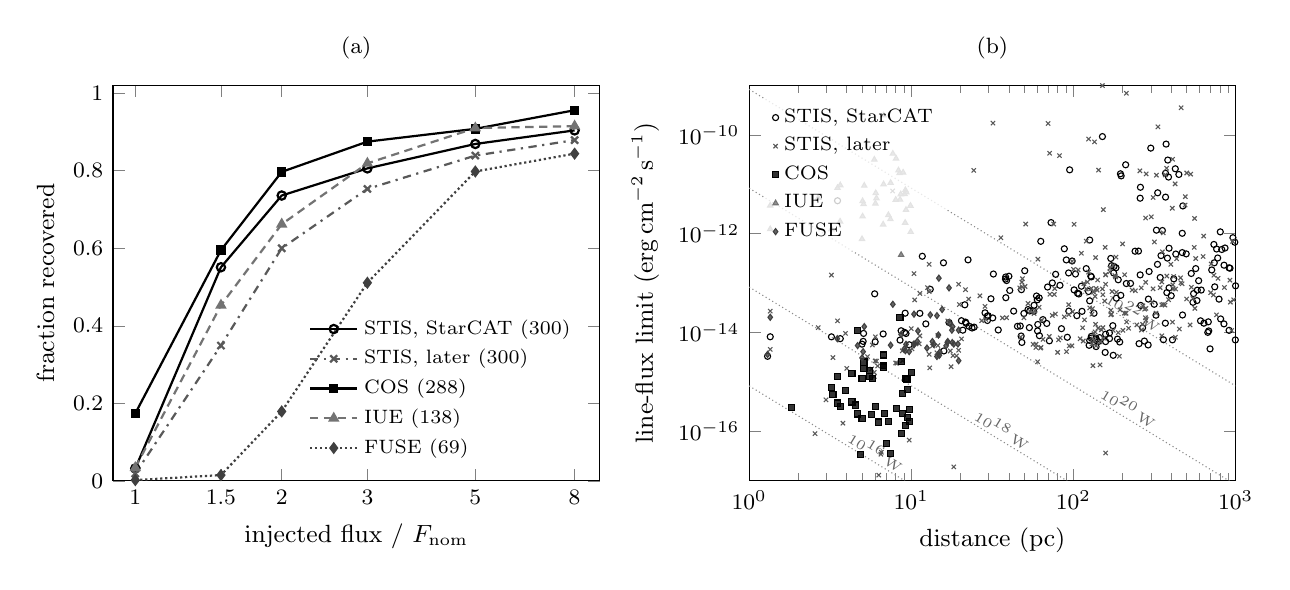
\begin{tikzpicture}
\begin{semilogxaxis}[name=rec,width=0.47\textwidth,height=0.4\textwidth,xmin=0.9,xmax=9,ymin=0,ymax=1.02,
  xtick={1,1.5,2,3,5,8},xticklabels={$1$,$1.5$,$2$,$3$,$5$,$8$},minor xtick={},
  xlabel={injected flux / $F_{\mathrm{nom}}$},ylabel={fraction recovered},
  tick label style={font=\footnotesize},label style={font=\small},title={(a)},title style={font=\footnotesize},
  legend style={font=\scriptsize,at={(0.97,0.03)},anchor=south east,draw=none,fill=none},legend cell align=left]
\addplot[black,thick,solid,mark=o,mark size=1.5pt,mark options={solid}] coordinates {(1,0.032) (1.5,0.551) (2,0.736) (3,0.806) (5,0.869) (8,0.904)};
\addlegendentry{STIS, StarCAT ($300$)}
\addplot[black!65,thick,dashdotted,mark=x,mark size=1.8pt,mark options={solid}] coordinates {(1,0.019) (1.5,0.349) (2,0.600) (3,0.753) (5,0.839) (8,0.879)};
\addlegendentry{STIS, later ($300$)}
\addplot[black,thick,solid,mark=square*,mark size=1.3pt,mark options={solid}] coordinates {(1,0.174) (1.5,0.595) (2,0.797) (3,0.875) (5,0.908) (8,0.956)};
\addlegendentry{COS ($288$)}
\addplot[black!55,thick,densely dashed,mark=triangle*,mark size=1.6pt,mark options={solid}] coordinates {(1,0.034) (1.5,0.453) (2,0.662) (3,0.819) (5,0.910) (8,0.915)};
\addlegendentry{IUE ($138$)}
\addplot[black!75,thick,densely dotted,mark=diamond*,mark size=1.6pt,mark options={solid}] coordinates {(1,0.002) (1.5,0.015) (2,0.179) (3,0.511) (5,0.798) (8,0.844)};
\addlegendentry{FUSE ($69$)}
\end{semilogxaxis}
\begin{loglogaxis}[at={(rec.east)},anchor=west,xshift=1.9cm,width=0.47\textwidth,height=0.4\textwidth,
  xmin=1,xmax=1000,ymin=1e-17,ymax=1e-9,xlabel={distance (pc)},ylabel={line-flux limit (\flux)},
  tick label style={font=\footnotesize},label style={font=\small},title={(b)},title style={font=\footnotesize},
  legend style={font=\scriptsize,at={(0.03,0.97)},anchor=north west,draw=none,fill=white,fill opacity=0.8,
  text opacity=1},legend cell align=left]
\addplot[only marks,mark=o,mark size=1.1pt,black] coordinates {(1.3,3.31e-15) (1.35,8.23e-15) (3.22,8.2e-15) (3.51,4.65e-12) (3.65,7.55e-15) (4.97,5.84e-15) (5.05,6.64e-15) (5.08,9.62e-15) (5.95,6.08e-14) (5.99,6.5e-15) (6.71,9.39e-15) (8.53,7.04e-15) (8.66,1.09e-14) (9.09,1.01e-14) (9.17,2.47e-14) (9.28,9.59e-15) (9.71,5.67e-15) (11.3,2.45e-14) (11.7,3.5e-13) (12.3,1.5e-14) (13.1,7.5e-14) (15.8,2.58e-13) (15.9,4.26e-15) (17.1,1.6e-14) (20.4,1.74e-14) (20.8,1.12e-14) (21.4,3.65e-14) (21.6,1.63e-14) (21.8,1.54e-14) (22.4,2.96e-13) (22.7,1.34e-14) (23.7,1.24e-14) (24.4,1.29e-14) (28.5,2.51e-14) (29.4,2.14e-14) (29.5,1.76e-14) (29.8,2.19e-14) (31,4.83e-14) (31.8,1.98e-14) (32.1,1.53e-13) (34.4,1.13e-14) (38.1,1.21e-13) (38.2,1.33e-13) (38.3,5.08e-14) (38.7,1.13e-13) (40,1.38e-13) (40.5,7.12e-14) (42.8,2.72e-14) (45.2,1.34e-14) (47,1.36e-14) (47.6,8.52e-15) (47.8,7.38e-14) (48.1,6.32e-15) (49.5,2.44e-14) (50.1,1.78e-13) (52.5,2.92e-14) (53.5,1.26e-14) (53.8,2.74e-14) (56.9,2.69e-14) (57.2,3.57e-14) (59.2,5.5e-14) (59.9,4.6e-14) (60.1,1.08e-14) (60.3,1.46e-14) (61.5,5.04e-14) (61.7,8.66e-15) (62.9,7.02e-13) (64.9,1.83e-14) (68.5,1.53e-14) (69.3,8.35e-14) (71.1,6.81e-15) (72.8,1.68e-12) (74.1,1.01e-13) (77.7,1.51e-13) (82.6,9.04e-14) (84.4,1.2e-14) (87.9,4.96e-13) (90.4,2.95e-13) (91.7,8.04e-15) (93.4,1.61e-13) (93.7,2.72e-14) (94.8,1.96e-11) (98.2,2.81e-13) (101,7.31e-14) (103,1.53e-13) (105,2.2e-14) (106,6.26e-14) (108,6.04e-14) (112,8.67e-14) (113,2.69e-14) (120,1.97e-13) (124,6.78e-14) (125,5.53e-15) (126,4.39e-14) (126,7.46e-13) (126,6.94e-15) (128,1.39e-13) (129,1.34e-13) (129,8.39e-15) (129,7.73e-15) (134,2.46e-14) (138,7.61e-15) (138,7.19e-15) (138,5.21e-15) (142,6.55e-15) (145,7.91e-15) (151,9.23e-11) (157,3.97e-15) (158,9.28e-15) (158,6.58e-15) (167,7.56e-15) (167,9.87e-15) (170,3.16e-13) (172,2.26e-13) (175,1.38e-14) (176,3.47e-15) (177,1.61e-13) (178,2.18e-13) (183,2.05e-13) (184,4.97e-14) (187,7.38e-15) (189,1.17e-13) (193,6.45e-15) (195,1.63e-11) (196,5.67e-14) (197,1.48e-11) (210,2.48e-11) (212,9.82e-14) (225,9.88e-14) (240,4.43e-13) (252,4.45e-13) (254,5.97e-15) (258,1.47e-13) (258,5.23e-12) (259,8.7e-12) (260,3.54e-14) (267,1.25e-14) (274,6.74e-15) (289,5.62e-15) (290,4.76e-14) (293,1.72e-13) (300,5.39e-11) (315,3.74e-14) (323,2.25e-14) (325,1.18e-12) (330,2.4e-13) (331,6.73e-12) (343,1.3e-13) (347,3.61e-13) (354,1.16e-12) (359,7.17e-15) (369,1.55e-14) (370,5.5e-12) (370,1.67e-11) (373,6.5e-11) (377,6.44e-14) (380,3.21e-13) (382,3.09e-11) (386,1.4e-11) (389,5.09e-13) (389,8.03e-14) (401,5.56e-14) (408,7.13e-15) (416,1.22e-13) (425,2.06e-11) (428,3.88e-13) (447,1.58e-11) (469,1.02e-12) (469,4.15e-13) (471,2.27e-14) (473,3.65e-12) (496,3.91e-13) (533,1.57e-13) (546,4.1e-14) (551,6.14e-14) (568,1.97e-13) (578,4.44e-14) (581,7.22e-14) (592,1.12e-13) (608,1.73e-14) (614,7.25e-14) (638,1.55e-14) (674,1.01e-14) (679,1.65e-14) (683,1.08e-14) (696,4.68e-15) (713,1.85e-13) (735,6.07e-13) (739,2.58e-13) (744,8.42e-14) (764,4.91e-13) (776,3.23e-13) (791,4.75e-14) (805,1.09e-12) (809,1.89e-14) (822,4.8e-13) (848,1.5e-14) (849,2.31e-13) (861,5.14e-13) (912,1.11e-14) (912,2.04e-13) (924,2.01e-13) (963,8.31e-13) (989,6.74e-13) (997,7.11e-15) (1e+03,8.84e-14) (1.04e+03,1.26e-13) (1.18e+03,3.07e-13) (1.19e+03,4.26e-13) (1.22e+03,2.28e-13) (1.36e+03,1.34e-13) (1.37e+03,9.16e-14) (1.43e+03,9.73e-13) (1.46e+03,5.54e-14) (1.52e+03,2.23e-14) (1.54e+03,7.24e-14) (1.55e+03,2.09e-12) (1.6e+03,6.67e-14) (1.62e+03,1.27e-14) (1.66e+03,1.34e-13) (1.67e+03,6.14e-15) (1.7e+03,1.24e-13) (1.74e+03,7.58e-13) (1.76e+03,5.22e-14) (1.8e+03,1.95e-13) (1.84e+03,3.09e-13) (1.86e+03,2.05e-13) (1.92e+03,7.83e-13) (1.97e+03,2.16e-13) (1.99e+03,7.76e-13) (2.01e+03,2.82e-13) (2.04e+03,2.19e-13) (2.05e+03,8.47e-14) (2.07e+03,4.99e-13) (2.17e+03,5.51e-13) (2.17e+03,6.05e-15) (2.2e+03,3.53e-13) (2.24e+03,4.99e-14) (2.25e+03,2.37e-14) (2.26e+03,1.12e-13) (2.28e+03,4.48e-13) (2.31e+03,7.95e-13) (2.32e+03,1.98e-13) (2.41e+03,8.87e-13) (2.44e+03,3.22e-13) (2.44e+03,1.4e-13) (2.48e+03,4.75e-14) (2.53e+03,5.5e-14) (2.54e+03,4.48e-14) (2.56e+03,2.5e-13) (2.71e+03,5.42e-14) (2.93e+03,3.92e-14) (3.12e+03,7.22e-13) (3.13e+03,3.47e-13) (3.54e+03,2.07e-13) (3.63e+03,3.84e-14) (3.69e+03,5.77e-14) (3.74e+03,3.31e-14) (3.97e+03,6.16e-14) (4.2e+03,4.49e-15) (4.42e+03,7.94e-14) (4.57e+03,1.03e-13) (4.64e+03,4.42e-14) (4.76e+03,7.82e-15) (4.93e+03,2.39e-14) (5.39e+03,1.22e-14) (5.62e+03,3.54e-14) (6.23e+03,2.43e-14) (6.24e+03,3.31e-15) (6.28e+03,1.68e-14) (6.31e+03,3.11e-14) (7.01e+03,2.14e-14) (7.31e+03,3.47e-14) (8.67e+03,5.65e-15) (8.94e+03,3.61e-14) (1.2e+04,2.53e-14) (1.64e+04,9.95e-14) (2.58e+04,2.14e-14) (3.08e+04,2.12e-14) (4.35e+04,3.5e-14) (4.44e+04,5.74e-14) (4.9e+04,4.88e-14) (6.29e+04,1.18e-13) (1e+05,4.14e-14) (1.04e+05,6.19e-15) (1.25e+05,2.16e-14) (2.5e+05,3.81e-14) (3.12e+05,3.5e-14) (3.57e+05,2.34e-14) (6.25e+05,1.39e-14) (9.09e+05,2.89e-14)};
\addlegendentry{STIS, StarCAT}
\addplot[only marks,mark=x,mark size=1.1pt,black!65,fill opacity=0.8] coordinates {(1.35,4.58e-15) (1.35,2.71e-14) (2.55,9.02e-17) (2.67,1.26e-14) (2.98,4.37e-16) (3.22,1.46e-13) (3.29,3.13e-15) (3.51,1.73e-14) (3.79,1.47e-16) (3.93,9.62e-15) (4,1.89e-15) (5.37,3.26e-15) (5.7,1.84e-15) (5.76,5.61e-15) (5.91,1.56e-15) (5.92,1.3e-15) (5.99,2.67e-15) (6.01,8.22e-15) (6.1,2.65e-15) (6.2,2.11e-15) (6.3,1.31e-17) (6.49,3.46e-17) (6.54,3.79e-17) (7.68,7.33e-12) (8.02,2.43e-15) (8.16,2.4e-15) (8.81,4.27e-15) (8.84,2.7e-15) (9.71,6.68e-17) (10,1.2e-14) (10.1,4.7e-15) (10.4,5.91e-15) (10.4,1.56e-13) (10.5,4.58e-14) (11.2,5.89e-15) (11.3,8.59e-15) (11.3,6.2e-14) (12.6,8.1e-14) (12.9,3.64e-15) (12.9,2.41e-13) (12.9,6.77e-14) (13,1.93e-15) (13.5,5.34e-15) (14.4,3.91e-15) (14.6,8.79e-15) (14.6,5.49e-15) (14.7,3.45e-15) (16.8,1.72e-14) (17.4,4.25e-15) (17.6,2.04e-15) (18.1,3.42e-15) (18.3,1.92e-17) (19,3.38e-15) (19.6,4.38e-15) (19.6,9.51e-14) (19.8,3.69e-14) (20.4,7.46e-15) (21.6,7.37e-14) (22.6,4.77e-14) (24.3,1.91e-11) (26.5,5.54e-14) (27.2,1.74e-14) (28.5,3.39e-14) (28.8,1.85e-14) (31.9,1.73e-10) (35.7,8.3e-13) (36.5,1.98e-14) (38.7,2e-14) (46.7,8e-14) (47.3,8.15e-15) (48.1,1.05e-13) (48.4,8.4e-14) (48.5,1.23e-13) (49.5,1.99e-14) (50.3,8.56e-14) (50.8,1.57e-12) (52.5,3.88e-14) (54.2,2.68e-14) (56.4,5.8e-15) (57.2,2.43e-14) (57.9,2.76e-14) (58.7,5.01e-15) (58.8,5.81e-15) (60.1,2.57e-15) (60.4,3.06e-13) (61.5,3.25e-14) (62.7,4.87e-15) (63.1,5.01e-15) (63.8,1.78e-14) (64.9,7.3e-15) (69.8,1.7e-10) (71,8.36e-15) (71.3,4.25e-11) (71.6,5.96e-14) (74.1,2.22e-14) (75.6,1.57e-12) (76.2,5.9e-14) (76.7,7.79e-14) (77.4,2.38e-14) (79.9,3.98e-15) (81,7.12e-15) (82,3.8e-11) (82.9,7.83e-15) (87.9,2.08e-14) (90.7,4.13e-15) (93.5,3.67e-14) (93.7,2.31e-14) (94.2,5.38e-15) (97.9,5.39e-15) (98.2,2.78e-13) (99,2.64e-14) (100,1.9e-13) (101,1.55e-12) (107,1.85e-13) (110,7.51e-15) (112,4.02e-13) (112,7.84e-18) (114,1.25e-14) (115,6.76e-15) (116,9.79e-14) (117,1.81e-14) (120,7.61e-14) (120,7.09e-13) (122,1.05e-13) (124,1.68e-13) (124,8.24e-11) (126,3.16e-14) (129,7.82e-14) (130,5.9e-15) (130,2.36e-14) (131,3.05e-14) (132,7.47e-15) (132,2.14e-15) (133,6.63e-14) (134,6.9e-15) (134,9.52e-15) (135,7.2e-11) (136,1.03e-14) (136,5.38e-14) (137,3.29e-13) (137,1.47e-14) (138,5.4e-15) (138,7.82e-14) (140,7.23e-14) (141,1.16e-13) (142,1.23e-14) (143,1.94e-11) (146,6.51e-15) (146,2.22e-15) (149,1.14e-14) (151,7.64e-14) (151,9.93e-10) (152,5.84e-14) (152,1.26e-14) (153,7.74e-15) (153,3.07e-12) (156,4.35e-14) (157,5.3e-13) (158,3.67e-17) (158,9.52e-14) (158,1.5e-13) (158,1.46e-13) (168,1.7e-13) (168,2e-13) (170,2.28e-14) (170,2.83e-14) (172,2.34e-14) (173,6.77e-14) (176,2.3e-13) (176,1.11e-14) (181,1.41e-13) (182,1.34e-13) (183,3.37e-13) (184,6.55e-14) (189,1e-14) (192,3.32e-15) (194,2.89e-14) (201,6.22e-13) (202,1.11e-14) (206,2.47e-14) (207,1.48e-13) (211,2.46e-14) (212,6.95e-10) (213,1.64e-14) (219,1.22e-14) (230,7.28e-14) (241,7.02e-14) (246,1.43e-14) (257,1.87e-11) (262,8.05e-14) (263,1.13e-14) (267,1.47e-14) (268,3.47e-14) (275,2.98e-14) (278,2e-14) (279,2.08e-12) (279,1.04e-13) (280,1.78e-14) (280,3.09e-14) (281,1.62e-11) (302,2.2e-12) (305,4.13e-14) (310,5.41e-12) (310,7.67e-14) (316,6.81e-13) (323,2.47e-14) (325,1.53e-11) (332,1.45e-10) (343,8.1e-14) (351,3.64e-14) (351,1.06e-13) (351,8.6e-15) (354,4.3e-13) (358,1.04e-12) (359,3.72e-14) (367,3.61e-14) (369,1.55e-11) (376,2.11e-11) (377,1.39e-13) (386,4.62e-14) (399,2.4e-13) (407,3.28e-12) (408,1.63e-14) (409,3.2e-11) (410,9.26e-14) (412,7.66e-14) (415,1.36e-13) (424,1.02e-11) (425,8.04e-15) (427,7.6e-14) (433,3.12e-13) (450,1.18e-14) (458,1.28e-13) (460,1.02e-13) (462,3.53e-10) (468,9.72e-14) (488,3.8e-12) (490,5.62e-12) (499,4.79e-14) (500,1.69e-11) (524,1.43e-14) (529,1.6e-11) (534,8.25e-14) (546,4.91e-14) (556,5.3e-13) (559,2.04e-12) (561,3.09e-14) (568,3.15e-13) (631,3.47e-13) (636,8.96e-13) (702,6.43e-14) (707,2.44e-13) (731,5.77e-14) (735,1.45e-13) (763,2.28e-14) (780,1.25e-13) (854,8.17e-14) (923,1.15e-13) (929,4.13e-14) (946,1.1e-14) (959,7.01e-13) (973,4.6e-14) (1.01e+03,1.96e-13) (1.01e+03,1.94e-12) (1.06e+03,6.04e-14) (1.07e+03,5.52e-15) (1.12e+03,1.96e-13) (1.12e+03,2.99e-13) (1.13e+03,1.18e-14) (1.14e+03,1.56e-14) (1.15e+03,7.85e-13) (1.16e+03,4.02e-12) (1.23e+03,1.35e-11) (1.25e+03,9.52e-15) (1.25e+03,7.61e-13) (1.28e+03,6e-14) (1.29e+03,7.02e-15) (1.3e+03,9.62e-14) (1.31e+03,4.99e-13) (1.31e+03,4.25e-14) (1.34e+03,3.06e-14) (1.37e+03,1.05e-13) (1.41e+03,1.22e-13) (1.42e+03,5.33e-14) (1.42e+03,5.5e-13) (1.44e+03,1.92e-13) (1.48e+03,9.86e-13) (1.52e+03,2.88e-14) (1.55e+03,1.46e-13) (1.55e+03,4.82e-13) (1.56e+03,1.03e-12) (1.57e+03,3.75e-13) (1.62e+03,3.89e-13) (1.62e+03,1.84e-13) (1.63e+03,4.99e-14) (1.68e+03,5.35e-13) (1.69e+03,2.97e-13) (1.69e+03,4.72e-13) (1.7e+03,1.31e-13) (1.83e+03,4.85e-14) (1.86e+03,2.87e-13) (1.91e+03,4.58e-14) (1.91e+03,8.34e-14) (1.92e+03,5.72e-13) (1.97e+03,2.71e-14) (1.97e+03,2.33e-13) (1.99e+03,2.89e-13) (2.01e+03,2.04e-13) (2.02e+03,2.43e-13) (2.06e+03,1.82e-13) (2.07e+03,2.88e-13) (2.17e+03,2.26e-13) (2.19e+03,2.49e-13) (2.2e+03,5.77e-13) (2.26e+03,1.61e-13) (2.31e+03,3.35e-13) (2.36e+03,2.24e-13) (2.41e+03,3.53e-13) (2.41e+03,4.45e-13) (2.42e+03,1.25e-13) (2.43e+03,1.82e-13) (2.45e+03,5.17e-13) (2.48e+03,1.86e-13) (2.51e+03,3.29e-13) (2.51e+03,7.84e-14) (2.53e+03,1.58e-13) (2.55e+03,4.48e-14) (2.55e+03,2.01e-13) (2.56e+03,2.55e-13) (2.56e+03,4.27e-14) (2.63e+03,7.83e-14) (2.71e+03,3.42e-14) (2.88e+03,8.63e-15) (3.12e+03,2.61e-13) (3.13e+03,2.84e-13) (3.45e+03,1.15e-13) (3.73e+03,1.33e-13) (3.78e+03,9.84e-14) (3.99e+03,6.73e-15) (4.04e+03,2.3e-13) (4.21e+03,2.77e-14) (4.23e+03,5.69e-14) (4.62e+03,2.25e-13) (4.67e+03,3.67e-13) (4.71e+03,1.39e-13) (4.92e+03,2.83e-14) (5.19e+03,4.12e-14) (5.39e+03,4.59e-14) (5.55e+03,1.09e-13) (5.59e+03,5.55e-14) (5.69e+03,1.17e-13) (6.61e+03,3.99e-14) (7.06e+03,5.65e-14) (7.11e+03,4.83e-14) (7.31e+03,4.78e-14) (8.94e+03,4.52e-14) (9.65e+03,4.73e-14) (1.01e+04,4.88e-14) (1.25e+04,5.18e-14) (1.36e+04,4.6e-14) (1.44e+04,6.73e-14) (1.64e+04,9.72e-14) (2.03e+04,4.94e-14) (2.04e+04,2.26e-14) (2.09e+04,4.62e-14) (2.21e+04,4.29e-14) (2.23e+04,8.86e-14) (2.48e+04,3.86e-14) (2.49e+04,5.38e-14) (2.68e+04,5.31e-14) (2.72e+04,3.74e-14) (2.74e+04,4.55e-14) (2.76e+04,4.1e-14) (2.89e+04,4.43e-14) (2.94e+04,3.22e-14) (3.12e+04,4.13e-14) (3.22e+04,3.54e-14) (3.22e+04,7.44e-14) (3.33e+04,6.79e-14) (3.4e+04,1.29e-14) (3.53e+04,4.56e-14) (3.69e+04,5.14e-14) (3.69e+04,5.47e-14) (3.91e+04,4.02e-14) (3.95e+04,5.13e-14) (4.63e+04,6.97e-14) (4.67e+04,4.63e-14) (4.98e+04,3.86e-14) (5.29e+04,4.39e-14) (6.9e+04,4.53e-14) (7.52e+04,4.84e-14) (8e+04,6.27e-14) (8.62e+04,4.77e-14) (1.15e+05,9.93e-14) (1.27e+05,4.89e-14) (1.37e+05,1.17e-13) (1.64e+05,3.2e-14) (1.92e+05,1.1e-13) (2e+05,4.11e-14) (2.44e+05,3.45e-14) (3.85e+05,5.12e-14) (4.55e+05,2.34e-14) (6.25e+05,8.76e-14) (1e+06,3.15e-14)};
\addlegendentry{STIS, later}
\addplot[only marks,mark=square*,mark size=1.1pt,black,fill opacity=0.8] coordinates {(1.83,3.03e-16) (3.22,7.76e-16) (3.29,5.66e-16) (3.5,1.28e-15) (3.52,3.76e-16) (3.67,3.19e-16) (3.93,6.74e-16) (4.31,3.95e-16) (4.31,1.49e-15) (4.55,3.42e-16) (4.64,1.11e-14) (4.67,2.26e-16) (4.87,3.39e-17) (4.97,1.19e-15) (4.97,1.86e-16) (5.11,1.86e-15) (5.11,2.54e-15) (5.52,1.29e-15) (5.52,1.71e-15) (5.69,2.19e-16) (5.79,1.2e-15) (5.99,3.18e-16) (6.3,1.55e-16) (6.71,2.12e-15) (6.75,2.01e-15) (6.75,3.52e-15) (6.86,2.34e-16) (7.05,5.72e-17) (7.24,1.62e-16) (7.41,3.57e-17) (8.08,2.86e-16) (8.52,2.03e-14) (8.66,9.24e-17) (8.66,2.6e-15) (8.81,5.92e-16) (8.81,2.31e-16) (9.17,1.3e-16) (9.28,1.16e-15) (9.42,1.15e-15) (9.44,6.95e-16) (9.49,1.95e-16) (9.71,2.74e-16) (9.78,1.58e-16) (10,1.54e-15)};
\addlegendentry{COS}
\addplot[only marks,mark=triangle*,mark size=1.1pt,black!55,fill opacity=0.8] coordinates {(1.35,1.24e-12) (1.35,3.72e-12) (2.64,2.72e-09) (2.67,5.33e-12) (3.22,1.23e-12) (3.51,8.46e-12) (3.64,1.77e-12) (3.65,9.58e-12) (4.97,7.81e-13) (5.01,2.24e-12) (5.01,4.57e-12) (5.08,3.97e-12) (5.13,9.39e-12) (5.92,3.16e-11) (6.01,4.09e-12) (6.04,6.65e-12) (6.1,5.23e-12) (6.71,1.54e-12) (6.75,2.48e-10) (6.75,1e-11) (7.23,2.39e-12) (7.44,1.97e-12) (7.46,1.07e-11) (7.68,1.01e-09) (7.7,4.17e-11) (8.02,4.86e-12) (8.06,3.33e-11) (8.34,1.91e-11) (8.47,1.68e-11) (8.53,4.9e-12) (8.61,6.28e-12) (8.66,3.73e-13) (8.91,1.73e-11) (9.09,6.34e-12) (9.17,1.67e-12) (9.2,7.63e-12) (9.28,3.04e-12) (9.32,6.9e-12) (9.89,3.69e-12) (9.92,1.09e-12)};
\addlegendentry{IUE}
\addplot[only marks,mark=diamond*,mark size=1.1pt,black!75,fill opacity=0.8] coordinates {(1.3,3.62e-15) (1.35,2.04e-14) (3.5,7.54e-15) (4.67,5.46e-15) (4.97,3.08e-15) (5.05,4.11e-15) (5.13,1.32e-14) (7.46,5.57e-15) (7.7,3.74e-14) (8.66,9.16e-15) (9.07,4.72e-15) (9.2,4.3e-15) (9.28,5.78e-15) (9.71,4.13e-15) (10.4,5.66e-15) (10.4,5.9e-15) (10.4,2.36e-14) (10.9,6.65e-15) (11,1.08e-14) (12.5,4.86e-15) (13.1,2.28e-14) (13.5,6.59e-15) (13.8,5.81e-15) (14.4,2.2e-14) (14.4,3.28e-15) (14.7,8.93e-15) (14.8,1.26e-13) (14.9,3.47e-15) (15,4.05e-15) (15.5,2.93e-14) (16.4,5.41e-15) (16.7,6.34e-15) (16.8,6.58e-15) (17.1,8.03e-14) (17.3,1.54e-14) (17.8,1.12e-14) (17.9,6.28e-15) (18,1.32e-14) (18.3,5.87e-15) (19.4,5.86e-15) (19.6,1.12e-14) (19.6,2.7e-15)};
\addlegendentry{FUSE}
\addplot[densely dotted,black!45,domain=1:9.142,samples=2,forget plot] {1e23/(4*pi*(x*3.0857e18)^2)} node[pos=0.78,sloped,above,font=\tiny,text=black!60,inner sep=1pt] {$10^{16}$\,W};
\addplot[densely dotted,black!45,domain=1:91.42,samples=2,forget plot] {1e25/(4*pi*(x*3.0857e18)^2)} node[pos=0.78,sloped,above,font=\tiny,text=black!60,inner sep=1pt] {$10^{18}$\,W};
\addplot[densely dotted,black!45,domain=1:914.2,samples=2,forget plot] {1e27/(4*pi*(x*3.0857e18)^2)} node[pos=0.78,sloped,above,font=\tiny,text=black!60,inner sep=1pt] {$10^{20}$\,W};
\addplot[densely dotted,black!45,domain=1:1000,samples=2,forget plot] {1e29/(4*pi*(x*3.0857e18)^2)} node[pos=0.78,sloped,above,font=\tiny,text=black!60,inner sep=1pt] {$10^{22}$\,W};
\end{loglogaxis}
\end{tikzpicture}
\caption{(a)~The fraction of injected lines recovered against their flux in units of
each exposure's nominal threshold, with the number of exposures in brackets.
(b)~Each star's limit on an unresolved line against its distance, with dotted lines of
constant isotropic luminosity.}
\label{fig:sens}
\end{figure}

\begin{table}[t]
\centering\small
\setlength{\tabcolsep}{5pt}
\caption{The best limit at each star within $5$\,pc. $\lambda$ is the median wavelength
of the spectra that give it, $F$ the line flux at the Earth, $L=4\pi d^2F$ the luminosity
of an isotropic source and $P_{10\,\mathrm{m}}$ the power of a transmitter aimed at
Earth through a diffraction-limited $10$\,m aperture.}
\label{tab:nearest}
\begin{tabular}{@{}lrlrlll@{}}
\toprule
Star & $d$ (pc) & Instrument & $\lambda$ (\AA) & $F$ (\flux) & $L$ (W) & $P_{10\,\mathrm{m}}$ (W)\\
\midrule
Proxima Centauri & $1.30$ & STIS & $1391$ & $3.3\times10^{-15}$ & $6.7\times10^{16}$ & $1.0\times10^{0}$\\
$\alpha$~Cen~A & $1.35$ & STIS & $1412$ & $8.2\times10^{-15}$ & $1.8\times10^{17}$ & $2.8\times10^{0}$\\
$\alpha$~Cen~B & $1.35$ & STIS, later & $1384$ & $4.6\times10^{-15}$ & $9.9\times10^{16}$ & $1.5\times10^{0}$\\
Barnard's star & $1.83$ & COS & $1212$ & $3.0\times10^{-16}$ & $1.2\times10^{16}$ & $1.4\times10^{-1}$\\
Lalande~21185 & $2.55$ & STIS, later & $1379$ & $9.0\times10^{-17}$ & $7.0\times10^{15}$ & $1.1\times10^{-1}$\\
Sirius~A & $2.64$ & IUE & $1563$ & $2.7\times10^{-9}$ & $2.3\times10^{23}$ & $4.4\times10^{6}$\\
Sirius~B & $2.67$ & STIS, later & $2826$ & $1.3\times10^{-14}$ & $1.1\times10^{18}$ & $6.8\times10^{1}$\\
Ross~154 & $2.98$ & STIS, later & $1379$ & $4.4\times10^{-16}$ & $4.6\times10^{16}$ & $7.0\times10^{-1}$\\
$\epsilon$~Eri & $3.22$ & COS & $1372$ & $7.8\times10^{-16}$ & $9.6\times10^{16}$ & $1.4\times10^{0}$\\
GJ~887 & $3.29$ & COS & $1586$ & $5.7\times10^{-16}$ & $7.3\times10^{16}$ & $1.5\times10^{0}$\\
61~Cyg~A & $3.50$ & COS & $1362$ & $1.3\times10^{-15}$ & $1.9\times10^{17}$ & $2.8\times10^{0}$\\
Procyon & $3.51$ & STIS, later & $1289$ & $1.7\times10^{-14}$ & $2.6\times10^{18}$ & $3.4\times10^{1}$\\
GJ~725~A & $3.52$ & COS & $1587$ & $3.8\times10^{-16}$ & $5.6\times10^{16}$ & $1.1\times10^{0}$\\
$\epsilon$~Ind & $3.64$ & IUE & $2991$ & $1.8\times10^{-12}$ & $2.8\times10^{20}$ & $2.0\times10^{4}$\\
$\tau$~Cet & $3.65$ & STIS & $1389$ & $7.5\times10^{-15}$ & $1.2\times10^{18}$ & $1.9\times10^{1}$\\
GJ~1061 & $3.67$ & COS & $1587$ & $3.2\times10^{-16}$ & $5.2\times10^{16}$ & $1.0\times10^{0}$\\
Luyten's star & $3.79$ & STIS, later & $1377$ & $1.5\times10^{-16}$ & $2.5\times10^{16}$ & $3.8\times10^{-1}$\\
Kapteyn's star & $3.93$ & COS & $1362$ & $6.7\times10^{-16}$ & $1.2\times10^{17}$ & $1.8\times10^{0}$\\
Kruger~60 & $4.00$ & STIS, later & $1380$ & $1.9\times10^{-15}$ & $3.6\times10^{17}$ & $5.5\times10^{0}$\\
GJ~628 & $4.31$ & COS & $1586$ & $4.0\times10^{-16}$ & $8.8\times10^{16}$ & $1.8\times10^{0}$\\
van Maanen's star & $4.31$ & COS & $1639$ & $1.5\times10^{-15}$ & $3.3\times10^{17}$ & $7.1\times10^{0}$\\
GJ~674 & $4.55$ & COS & $1217$ & $3.4\times10^{-16}$ & $8.5\times10^{16}$ & $1.0\times10^{0}$\\
LAWD~37 & $4.64$ & COS & $1668$ & $1.1\times10^{-14}$ & $2.9\times10^{18}$ & $6.3\times10^{1}$\\
GJ~876 & $4.67$ & COS & $1312$ & $2.3\times10^{-16}$ & $5.9\times10^{16}$ & $8.1\times10^{-1}$\\
DENIS~J0255$-$4700 & $4.87$ & COS & $1156$ & $3.4\times10^{-17}$ & $9.6\times10^{15}$ & $1.0\times10^{-1}$\\
AD~Leo & $4.97$ & COS & $1139$ & $1.2\times10^{-15}$ & $3.5\times10^{17}$ & $3.6\times10^{0}$\\
GJ~832 & $4.97$ & COS & $1312$ & $1.9\times10^{-16}$ & $5.5\times10^{16}$ & $7.5\times10^{-1}$\\
\bottomrule
\end{tabular}
\end{table}

% =============================================================================
\section{Related work}\label{sec:related}
% =============================================================================

\emph{Laser searches.} The searches of
Section~\ref{sec:intro}~\cite{ReinesMarcy2002,TellisMarcy2015,TellisMarcy2017,Zuckerman2023,FieldsGoodman2025}
look for unresolved lines in optical spectra from the ground, with thresholds of tens of
kilowatts to megawatts for a $10$\,m transmitter at the distances of their stars; the
HARPS search, like this one, finds that the features which survive its tests lie in
stars whose own spectra must be excluded first. We find no search of ultraviolet
spectra.

\emph{Ultraviolet spectra of nearby stars.} The archives were assembled to study
chromospheres, transition regions, winds and the interstellar medium. StarCAT collects
the STIS echelle spectra of $545$ stars~\cite{Ayres2010}, the pipeline's x1d files hold
the later ones, and the COS spectra of nearby M
dwarfs come largely from programmes that measure their ultraviolet radiation for the
atmospheres of their planets~\cite{France2016}. These are the deepest ultraviolet spectra
of the nearest stars, and the narrow emission lines they reveal, such as the
\ion{Fe}{ii} lines that follow \ion{Mg}{ii} through the pulsation of Mira
variables~\cite{WoodKarovska2000}, are what an unresolved feature must be told apart
from.

% =============================================================================
\section{Conclusion}\label{sec:conclusion}
% =============================================================================

No unresolved ultraviolet emission line that a laser aimed at Earth could produce is
found in the STIS, COS, IUE and FUSE spectra of nearby stars. Every feature that persists
in one star and that the tests against other stars do not remove belongs to the spectrum
of an evolved star or is a chromospheric line of $\epsilon$~Eri, and at the nearest stars
a transmitter of about a watt behind a $10$\,m aperture, its beam held on the Earth,
would have been seen, from $21$ of the $27$ stars within $5$\,pc.

The limits apply to lines that are steady or recur in the spectra of a star, that rise
above the local upper envelope and that lie away from the masked lines, and to the
epochs of the archival spectra. A laser at the wavelength of a strong stellar line, one
in an evolved star whose spectrum holds narrow emission lines, or one that was off when
the spectra were taken is not constrained. The COS spectra of the stars beyond $10$\,pc
remain to be searched.

\section*{Acknowledgements}

This work is based on observations made with the NASA/ESA Hubble Space Telescope,
obtained from the Mikulski Archive for Space Telescopes (MAST) at the Space Telescope
Science Institute, which is operated by the Association of Universities for Research in
Astronomy, Inc., under NASA contract NAS~5-26555, and on IUE and FUSE data from MAST. It
uses the StarCAT catalogue, the SIMBAD database, operated at CDS, Strasbourg, France,
and the NIST Atomic Spectra Database, and the software Astropy~\cite{Astropy2022},
NumPy~\cite{Harris2020} and SciPy~\cite{Virtanen2020}.

\begin{thebibliography}{99}\small\raggedright
\setlength{\itemsep}{1pt}

\bibitem{SchwartzTownes1961}
R.~N. Schwartz and C.~H. Townes, Interstellar and interplanetary communication by
optical masers, \emph{Nature} \textbf{190}, 205 (1961).

\bibitem{ReinesMarcy2002}
A.~E. Reines and G.~W. Marcy, Optical search for extraterrestrial intelligence: a
spectroscopic search for laser emission from nearby stars, \emph{Publ. Astron. Soc.
Pac.} \textbf{114}, 416 (2002).

\bibitem{TellisMarcy2015}
N.~K. Tellis and G.~W. Marcy, A search for optical laser emission using Keck HIRES,
\emph{Publ. Astron. Soc. Pac.} \textbf{127}, 540 (2015).

\bibitem{TellisMarcy2017}
N.~K. Tellis and G.~W. Marcy, A search for laser emission with megawatt thresholds from
5600 FGKM stars, \emph{Astron. J.} \textbf{153}, 251 (2017).

\bibitem{Zuckerman2023}
A.~Zuckerman, Z.~Ko, H.~Isaacson, et al., The Breakthrough Listen search for
intelligent life: a laser search pipeline for the Automated Planet Finder,
\emph{Astron. J.} \textbf{165}, 114 (2023).

\bibitem{FieldsGoodman2025}
B.~Fields and J.~C. Goodman, A 2821 star optical SETI survey using ESO HARPS archival
data, arXiv:2508.08628 (2025).

\bibitem{Hinkle2005}
K.~Hinkle, L.~Wallace, J.~Valenti and T.~Ayres, \emph{Ultraviolet Atlas of the Arcturus
Spectrum, 1150--3800\,\AA} (Astronomical Society of the Pacific, San Francisco, 2005).

\bibitem{RedfieldLinsky2008}
S.~Redfield and J.~L. Linsky, The structure of the local interstellar medium. IV.
Dynamics, morphology, physical properties, and implications of cloud-cloud
interactions, \emph{Astrophys. J.} \textbf{673}, 283 (2008).

\bibitem{Woodgate1998}
B.~E. Woodgate, R.~A. Kimble, C.~W. Bowers, et al., The Space Telescope Imaging
Spectrograph design, \emph{Publ. Astron. Soc. Pac.} \textbf{110}, 1183 (1998).

\bibitem{Ayres2010}
T.~R. Ayres, StarCAT: a catalog of Space Telescope Imaging Spectrograph ultraviolet
echelle spectra of stars, \emph{Astrophys. J. Suppl. Ser.} \textbf{187}, 149 (2010).

\bibitem{Green2012}
J.~C. Green, C.~S. Froning, S.~Osterman, et al., The Cosmic Origins Spectrograph,
\emph{Astrophys. J.} \textbf{744}, 60 (2012).

\bibitem{Boggess1978}
A.~Boggess, F.~A. Carr, D.~C. Evans, et al., The IUE spacecraft and instrumentation,
\emph{Nature} \textbf{275}, 372 (1978).

\bibitem{NicholsLinsky1996}
J.~S. Nichols and J.~L. Linsky, The final archive and recalibration of the
International Ultraviolet Explorer (IUE) satellite, \emph{Astron. J.} \textbf{111}, 517
(1996).

\bibitem{Moos2000}
H.~W. Moos, W.~C. Cash, L.~L. Cowie, et al., Overview of the Far Ultraviolet
Spectroscopic Explorer mission, \emph{Astrophys. J.} \textbf{538}, L1 (2000).

\bibitem{Sahnow2000}
D.~J. Sahnow, H.~W. Moos, T.~B. Ake, et al., On-orbit performance of the Far
Ultraviolet Spectroscopic Explorer satellite, \emph{Astrophys. J.} \textbf{538}, L7
(2000).

\bibitem{Dixon2007}
W.~V. Dixon, D.~J. Sahnow, P.~E. Barrett, et al., CalFUSE version 3: a data reduction
pipeline for the Far Ultraviolet Spectroscopic Explorer, \emph{Publ. Astron. Soc. Pac.}
\textbf{119}, 527 (2007).

\bibitem{Wenger2000}
M.~Wenger, F.~Ochsenbein, D.~Egret, et al., The SIMBAD astronomical database,
\emph{Astron. Astrophys. Suppl. Ser.} \textbf{143}, 9 (2000).

\bibitem{NIST}
A.~Kramida, Yu.~Ralchenko, J.~Reader and NIST ASD Team, \emph{NIST Atomic Spectra
Database} (National Institute of Standards and Technology, Gaithersburg, 2024).

\bibitem{WoodKarovska2000}
B.~E. Wood and M.~Karovska, Studying the pulsation of Mira variables in the
ultraviolet, \emph{Astrophys. J.} \textbf{535}, 304 (2000).

\bibitem{France2016}
K.~France, R.~O.~P. Loyd, A.~Youngblood, et al., The MUSCLES Treasury Survey. I.
Motivation and overview, \emph{Astrophys. J.} \textbf{820}, 89 (2016).

\bibitem{Astropy2022}
Astropy Collaboration, A.~M. Price-Whelan, P.~L. Lim, et al., The Astropy Project:
sustaining and growing a community-oriented open-source project and the latest major
release (v5.0) of the core package, \emph{Astrophys. J.} \textbf{935}, 167 (2022).

\bibitem{Harris2020}
C.~R. Harris, K.~J. Millman, S.~J. van~der Walt, et al., Array programming with NumPy,
\emph{Nature} \textbf{585}, 357 (2020).

\bibitem{Virtanen2020}
P.~Virtanen, R.~Gommers, T.~E. Oliphant, et al., SciPy 1.0: fundamental algorithms for
scientific computing in Python, \emph{Nat. Methods} \textbf{17}, 261 (2020).

\end{thebibliography}

\end{document}
